\chapter{Usage}
\label{cha:Usage}

\begin{figure}[H]
\centering
	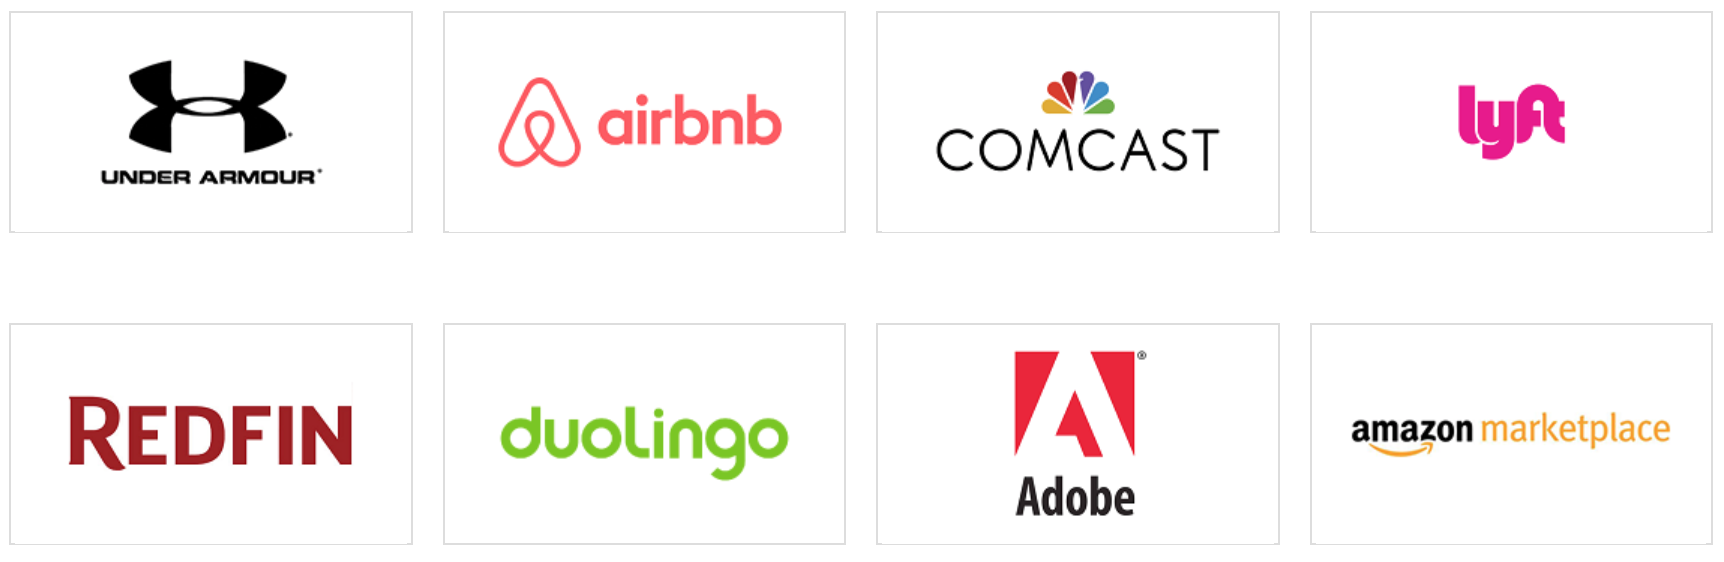
\includegraphics[width=0.99\textwidth]{images/customerstudies}
	\caption{short selection companies using DyanamoDB}
	\label{fig:usage}
\end{figure}

Figure \ref{fig:usage} is listing some of the bigger companies, which are known for using DynamoDB for various projects. \\

As Amazon is promoting on its own website, DynamoDB can for example be used for \textbf{Ad Tech}. It is mentioned, that recommendation engines or realtime bidding platforms are easy to implement because of DynamoDB's consistent, single-digit millisecond latency, that is delivered at any scale. 

When coming to Ad Tech, Amazon is referring to the company \textit{VidRoll}, which is currently using this NoSQL database to help match hundreds of millions appropriate video ads (per month) with site visitors across 100.000 websites.\cite{aws} \\

Another example is \textbf{Gaming}: Responsive games for desktop, console or mobile devices can store and query Amazon Lumberyard\footnote{Amazon Lumberyard is a free cross-platform AAA game engine. It is provided by Amazon, for further information please have a look at \href{https://aws.amazon.com/lumberyard/}{www.aws.amazon.com/lumberyard}} game data through Cloud Canvas\footnote{Cloud Canvas is a suite of tools and solutions, that is designed to achieve an easy implementation of cloud-connected features using on-demand, global storage and compute provided by AWS. For further information please have a look at \href{http://docs.aws.amazon.com/lumberyard/latest/developerguide/cloud-canvas-intro.html}{www.docs.aws.amazon.com/lumberyard/latest/developerguide/cloud-canvas-intro.html}}. DynamoDB can easily integrate with the AWS Mobile SDK\footnote{AWS Mobile SDK can help building app quickly and easily and has an easy access to many AWS services. It is available for iOS 8+, Android/Fire OS, Xamarin, Reactive Native, and many more. It is provided by Amazon, for further information please have a look at \href{https://aws.amazon.com/mobile/sdk/}{www.aws.amazon.com/mobile/sdk}} and other AWS services, for example for user authentication, social features or downloadable content.

A good example (and nice to mention) is \textit{Zynga Poker}, which just recently moved a MySQL farm over to Amazon DynamoDB and therefore reduced their operational overhead drastically.\cite{aws} \\

\textit{Canary} for example, is using AWS' scalability to support more than 150 million incoming videos daily within its home security systems. DynamoDB lets you connect your high-velocity, high-volume \textbf{IoT} data to a Amazon Redshift\footnote{Amazon Redshift is a fast, simple, fully-managed and cost-effective data warehouse. t is provided by Amazon, for further information please have a look at \href{https://aws.amazon.com/redshift/}{www.aws.amazon.com/redshift}}data warehouse to enable BI analysis.\cite{aws}\\

Of course, Amazon likes to tell how amazing DynamoDB is in nearly every use case. But because one can not simply rely on one company's own marketing information, let's have a look at some real life use cases from multiple websites and different people:\\


\section{Real Life Use Cases}

\vspace{10pt}
\begin{minipage}[t]{4cm}
\textbf{Michael L.} \\
		works at The Internet \\
		studied at Youtube \\
		thinks he is funny..\\
\end{minipage}
\hfill
\begin{minipage}[t]{10cm}
Says, that instead of storing php sessions on the server's local file system, a good use case would be to use DynamoDB when having a php site running on multiple ec2 servers managed by an Elastic Load Balancer.\cite{user-stories} \\
\end{minipage}

	
\vspace{20pt}


\hspace{-20pt}
\begin{minipage}[t]{9cm}
Camille tells, that at Clubhouse (\href{https://clubhouse.io}{www.clubhouse.io}), they use DynamoDB as a scalable backend for their Datomic database and DynamoDB Local in their local development environments.\cite{user-stories}\\
\end{minipage}
\hfill
\begin{minipage}[t]{4.5cm}
\textbf{Camille Emefa Acey}\\
works at Clubhouse Software Inc.\\
\end{minipage}

\vspace{20pt}

\hspace{-20pt}
\begin{minipage}[t]{4cm}
\textbf{Ben Darfler} \\
Systems Builder \\
\end{minipage}
\hfill
\begin{minipage}[t]{10cm}
Mentions, that at Localytics they decided to go with DynamoDB because they need to process data just once. And only once.\cite{user-stories} \\
\end{minipage}














